%%%%%%%%%%%%%%%%%%%%%%%%%%%%%%%%%%%%%%%%%%%%%%%%%%%%%%%%%%%%%
% Praca inżynierska — System zarządzania pracą drukarki 3D
% Oliwer Urbaniak, Uniwersytet Wrocławski
%%%%%%%%%%%%%%%%%%%%%%%%%%%%%%%%%%%%%%%%%%%%%%%%%%%%%%%%%%%%%

\documentclass[a4paper,12pt,reqno]{article}
%----------------------------------------------------------
\usepackage{amsfonts}
\usepackage{graphicx}
\usepackage{geometry}
\usepackage{color}
\usepackage{amssymb,amsmath}
\usepackage{polski}
\usepackage[T1]{fontenc}
\usepackage[utf8]{inputenc}
\usepackage{caption}
\geometry{margin=1.1in}
\usepackage{wrapfig}
\usepackage{lipsum}  
\usepackage{listings}
\usepackage[toc,page]{appendix}
\usepackage{url}
\usepackage{hyperref}
\usepackage{enumitem}
\usepackage{booktabs}
\usepackage{longtable}
\usepackage{array}
\usepackage{xcolor}

\definecolor{codegreen}{rgb}{0.5, 0.09, 0.09}
\definecolor{codegray}{rgb}{0.5,0.5,0.5}
\definecolor{codepurple}{rgb}{0.58,0,0.82}
\definecolor{backcolour}{rgb}{0.94,0.94,0.94}
\definecolor{gray}{rgb}{0,0.6,0}

\lstdefinestyle{mystyle}{
	backgroundcolor=\color{backcolour},
	commentstyle=\color{codegreen},
	keywordstyle=\color{codeblue},
	numberstyle=\tiny\color{codegray},
	stringstyle=\color{codepurple},
	basicstyle=\footnotesize\fontfamily{cmtt}\selectfont,
	breakatwhitespace=false,
	breaklines=true,
	captionpos=b,
	keepspaces=true,
	numbers=left,
	numbersep=5pt,
	showspaces=false,
	showstringspaces=false,
	showtabs=false,
	tabsize=2
}

\lstdefinestyle{jsonStyle}{
	backgroundcolor=\color{backcolour},
	commentstyle=\color{codegreen},
	keywordstyle=\color{codeblue},
	numberstyle=\tiny\color{codegray},
	stringstyle=\color{codepurple},
	basicstyle=\footnotesize\fontfamily{cmtt}\selectfont,
	breaklines=true,
	captionpos=b,
	keepspaces=true,
	numbers=left,
	numbersep=5pt,
	showspaces=false,
	showstringspaces=false,
	showtabs=false,
	tabsize=2
}
 
\lstset{style=mystyle}
\lstset{literate=%
    *{0}{{{\color{gray}0}}}1
    {1}{{{\color{gray}1}}}1
    {2}{{{\color{gray}2}}}1
    {3}{{{\color{gray}3}}}1
    {4}{{{\color{gray}4}}}1
    {5}{{{\color{gray}5}}}1
    {6}{{{\color{gray}6}}}1
    {7}{{{\color{gray}7}}}1
    {8}{{{\color{gray}8}}}1
    {9}{{{\color{gray}9}}}1
}
%------------------------------------------------------------
\begin{document}
	
% ============================================================
%  STRONA TYTUŁOWA
% ============================================================

%\begin{figure}[h]
%	\centering
%		
\includegraphics[width=0.40\textwidth]{logo.pdf}
%\end{figure}


\begin{center}

\thispagestyle{empty}

%UNIWERSYTET WROCŁAWSKI\\
\Large 
Uniwersytet Wrocławski\\
Wydział Fizyki i Astronomii\\
\vspace{0.8cm}
\vspace{1.8cm}

\Large Oliwer Urbaniak \\
\vspace{3.2cm}
\Large System zarządzania pracą drukarki 3D w laboratorium studenckim. \\

\end{center}
\vspace{5.5cm}
\begin{flushright}
\large{ Praca inżynierska na kierunku \\Informatyka Stosowana i Systemy Pomiarowe \\}
\vspace{0.5cm}
\large{ Opiekun \\ dr Bartosz Brzostowski}
\end{flushright}
\vspace{2.2cm}

\begin{center}
\large Wrocław, \today
\end{center}

\newpage

% ============================================================
%  SPIS TREŚCI
% ============================================================

\tableofcontents

\newpage
% ============================================================
%  STRESZCZENIE
% ============================================================
\begin{flushleft}
\Large \textbf{Streszczenie}
\end{flushleft}
\vspace{1cm}


Niniejsza praca inżynierska opisuje projekt, implementację oraz wykonanie systemu \textit{AddiPi} - rozproszonego systemu zarządzania pracą drukarki 3D przeznaczonego dla laboratorium studenckiego. System umożliwia użytkownikom przesyłanie plików G-code, planowanie oraz monitorowanie zadań do wydruku, a administratorom - pełną kontrolę nad kolejką i użytkownikami.

Architektura systemu oparta jest na podejściu mikroserwisowym. Wyodrębniono sześć niezależnych serwisów backendowych: uwierzytelniania (Auth Service), zarządzania użytkownikami (User Service), obsługi plików (Files Service), kolejkowania zadań (Queue Service), sterowania drukarką (Printer Service) oraz agenta działającego na urządzeniu Raspberry Pi (AddiPi Agent). Całość uzupełnia aplikacja frontendowa zbudowana w React oraz serwis wideo do podglądu kamery.

Komunikacja między serwisami odbywa się za pośrednictwem protokołu HTTP/REST oraz chmurowej kolejki Azure Service Bus. Dane przechowywane są w Azure Cosmos DB, a pliki G-code w Azure Blob Storage. Sterowanie drukarką realizowane jest przez Azure IoT Hub przy użyciu bezpośrednich wywołań metod (Direct Methods) na Raspberry Pi, na którym działa oprogramowane OctoPrint.

System zrealizowano przy użyciu języków TypeScript (Node.js) i Python. Wdrożenie odbywa się w kontenerach Docker, koordynowanych plikiem Docker Compose. Interfejs użytkownika obsługuje uwierzytelnianie tokenem JWT, przesyłanie plików, planowanie zadań, podgląd kamery w czasie rzeczywistym oraz panel administracyjny.

\vspace{0.3cm}
\textbf{Słowa kluczowe:} mikroserwisy, drukarka 3D, OctoPrint, Raspberry Pi, Azure Iot Hub, Azure Cosmos DB, Docker, TypeScript, Python, REST API, kolejkowanie zadań

\newpage

% ============================================================
%  ROZDZIAŁ 1 — WPROWADZENIE
% ============================================================

\section{Wprowadzenie}

\subsection{Motywacja i cel pracy}



Drukarki 3D stanowią obecnie standardowe wyposażenie laboratoriów akademickich, warsztatów studenckich oraz zakładów produkcyjnych zorientowanych na wytwarzanie przyrostowe. Urządzenia te, pomimo rosnącej dostępności i malejących cen, pozostają zasobem współdzielonym - ich liczba jest zwykle ograniczona, a czas drukowania pojedynczego modelu może wynosić od kilkunastu minut do wielu godzin. W środowisku akademickim oraz przemysłowym rodzi to naturalne problemy organizacyjne: konieczność ręcznego umawiania się na czas druku, brak przejrzystości stanu kolejki oraz niemożność zdalnego monitorowania postępu pracy.

Celem niniejszej pracy jest zaprojektowanie i implementacja systemu \textit{AddiPi}, który automatyzuje proces zarządzania drukarką 3D w laboratorium studenckim. System pozwala użytkownikom na:
\begin{itemize}
	\item przesyłanie plików G-code przez przeglądarkę internetową,
	\item planowanie druków na określony termin lub dodawanie ich do kolejki,
	\item śledzenie postępu druku w czasie rzeczywistym, wraz z podglądem kamery,
	\item otrzymywanie powiadomień o zakończeniu lub błędzie druku.
\end{itemize}


Administratorzy laboratorium zyskują natomiast narzędzia do zarządzania użytkownikami, przeglądania historii wszystkich zadań oraz sterowania kolejką i urządzeniami.

\subsection{Zakres pracy}

Praca obejmuje:
\begin{enumerate}
	\item analizę wymagań systemu i wybór technologii,
	\item projekt architektury mikroserwisowej,
	\item implementację wszystkich komponentów backendowych i frontendowych,
	\item konfigurację infrastruktury chmurowej (Microsoft Azure),
	\item wdrożenie systemu przy użyciu kontenerów Docker,
	\item testy poprawności działania.
\end{enumerate}

\subsection{Struktura pracy}

Rozdział~\ref{sec:analiza} zawiera analizę wymagań i przegląd istniejących rozwiązań. Rozdział~\ref{sec:technologie} omawia wybrane technologie i uzasadnia decyzje projektowe. Rozdział~\ref{sec:architektura} opisuje architekturę systemu. Rozdziały~\ref{sec:backend}--\ref{sec:agent} szczegółowo omawiają implementację poszczególnych komponentów programowych. Rozdział~\ref{sec:cad} opisuje projekt mechaniczny obudowy w SolidWorks. Rozdział~\ref{sec:rpi} omawia konfigurację Raspberry Pi, automatyzację przez cron i tunel Cloudflare. Rozdział~\ref{sec:wdrozenie} dotyczy wdrożenia i infrastruktury chmurowej Azure. Rozdział~\ref{sec:testy} przedstawia wyniki testów. Praca kończy się podsumowaniem w roziale~\ref{sec:podsumowanie}.

\newpage

% ============================================================
%  ROZDZIAŁ 2 — ANALIZA WYMAGAŃ
% ============================================================

\section{Analiza wymagań i przegląd rozwiązań}
\label{sec:analiza}

\subsection{Wymagania funkcjonalne}
 
W swojej pracy możesz odnosić się do równań np. do równania (\ref{rownanie}) lub do rysunków, zarówno wektorowych, patrz rys. (\ref{logotyp}) jak i bitmapowych (\ref{wahadla}).
Możesz też z powodzeniem cytować literaturę pojedynczo
\cite{Matyka2008} lub kilka pozycji na raz
\cite{Strzelczyk2021,Chorin1968}. Jeśli chcesz to robić wygodniej załóż tzw, plik bibtex, ale możesz też pracować tak, jak w tym dokumencie.



\begin{equation} 
\rho\left(\frac{\partial\vec v}{\partial t}+(\vec v\cdot\nabla)\vec v\right) =\rho\vec f - \nabla p + \mu\triangle\vec v, \label{rownanie}
\end{equation} 

Lorem ipsum dolor sit amet, consectetur adipiscing elit, sed do eiusmod tempor incididunt ut labore et dolore magna aliqua. Ut enim ad minim veniam, quis nostrud exercitation ullamco laboris nisi ut aliquip ex ea commodo consequat. Duis aute irure dolor in reprehenderit in voluptate velit esse cillum dolore eu fugiat nulla pariatur. Excepteur sint occaecat cupidatat non proident, sunt in culpa qui officia deserunt mollit anim id est laborum.





\begin{figure}[!ht]%
\centering

\includegraphics[scale=0.85]{logo.pdf}
\caption{Podpis rysunku, który jest obrazem wektorowym (EPS). \label{logotyp}}
\qquad
\end{figure}   




\begin{figure}[!ht]%
\centering
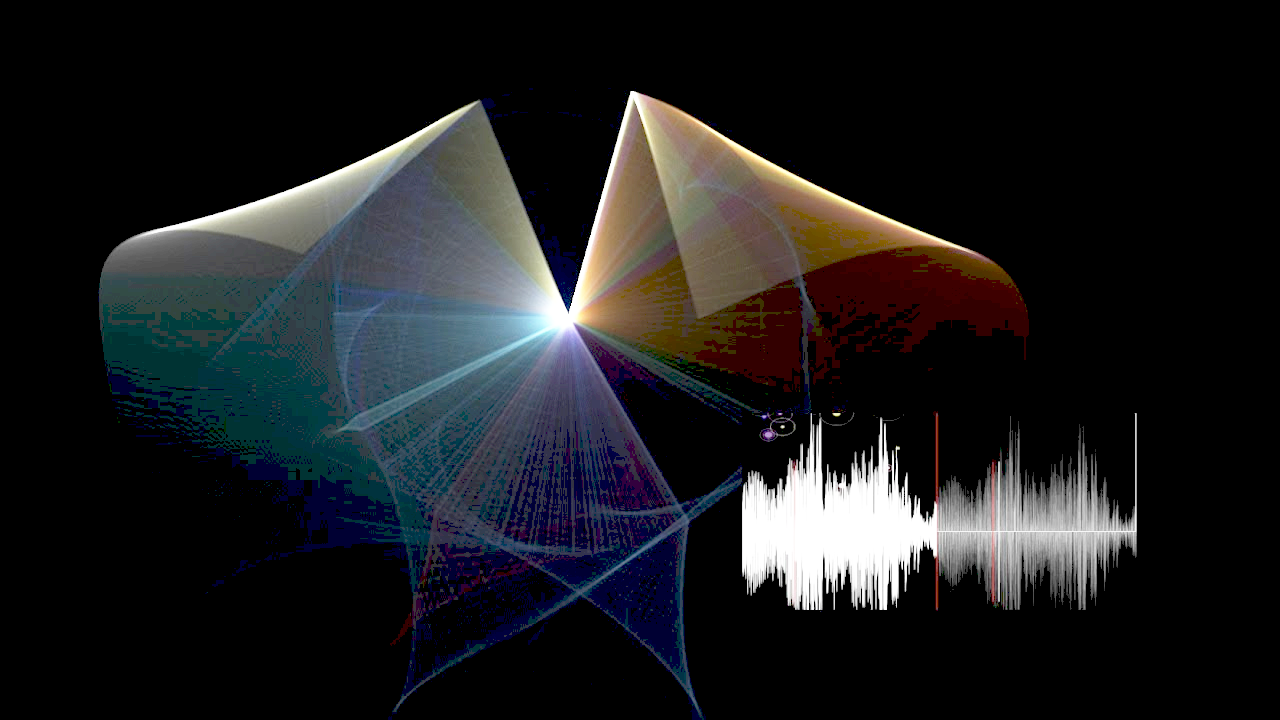
\includegraphics[width=0.8\columnwidth]{pendulums.png}
\caption{To jest rysunek drugi, kilkadziesiąt wahadeł podwójnych z syntezą dźwięku.\label{wahadla}}%
%
\qquad
\end{figure}


\subsection{Wymagania niefunkcjonalne}

Lorem ipsum dolor sit amet, consectetur adipiscing elit, sed do eiusmod tempor incididunt ut labore et dolore magna aliqua. Ut enim ad minim veniam, quis nostrud exercitation ullamco laboris nisi ut aliquip ex ea commodo consequat. Duis aute irure dolor in reprehenderit in voluptate velit esse cillum dolore eu fugiat nulla pariatur. Excepteur sint occaecat cupidatat non proident, sunt in culpa qui officia deserunt mollit anim id est laborum. \label{Rysunek14}
.. in the figure \ref{Rysunek14}.


\subsection{Przegląd istniejących rozwiązań}

\subsubsection{Octoprint}

\subsubsection{Mainsail i Fluidd}

\subsubsection{Rozwiązania komercyjne}

\subsubsection{Wnioski}

\newpage

% ============================================================
%  ROZDZIAŁ 3 — TECHNOLOGIE
% ============================================================

\section{Wybór technologii}
\label{sec:technologie}

\subsection{Języki programowania}

\subsubsection{TypeScript / Node.js}

\subsubsection{Python}


\subsection{Framework webowy - Express.js}

\subsection{Baza danych - Azure Cosmos DB}

\subsection{Przechowywanie plików - Azure Blob Storage}

\subsection{Kolejkowanie - Azure Service Bus}

\subsection{Sterowanie urządzeniem - Azure IoT Hub}

\subsection{Frontend - React i Vite}

\subsection{Kontenery - Docker i Docker Compose}

\subsection{CAD - SolidWorks}

\subsection{Porównanie wybranych alternatyw}

\newpage

% ============================================================
%  ROZDZIAŁ 4 — ARCHITEKTURA SYSTEMU
% ============================================================
\section{Architektura systemu}
\label{sec:architektura}

\subsection{Ogólna struktura}

\subsection{Diagram architektury}

\subsection{Model danych}

\subsubsection{Użytkownik (kontener \texttt{users})}

\subsubsection{Zadanie (kontener \texttt{jobs})}

\subsubsection{Refresh Token (kontener \texttt{refresh-token})}


\subsection{Cykl życia zadania do wydruku}

\subsection{Bezpieczeństwo i uwierzytelnianie}

\newpage

% ============================================================
%  ROZDZIAŁ 5 — IMPLEMENTACJA BACKENDU
% ============================================================
\section{Implementacja serwisów backendowych}
\label{sec:backend}

\subsection{Auth Service}

\subsubsection{Opis ogólny}

\subsubsection{Endpointy API}

\subsubsection{Kluczowe fragmenty implementacji}

\subsubsection{Weryfikacja e-mail}

\subsection{User Service}

\subsubsection{Opis ogólny}

\subsubsection{Endpointy API}

\subsubsection{Mechanizm autoryzacji}


\subsection{Files Service}

\subsubsection{Opis ogólny}

\subsubsection{Przepływ przesyłania pliku}


\subsection{Queue Service}

\subsubsection{Opis ogólny}

\subsubsection{Listener kolejki}

\subsubsection{Endpointy HTTP API}


\subsection{Printer Service}

\subsubsection{Opis ogólny}

\subsubsection{Harmonogram}

\subsubsection{Monitor gotowości}

\subsubsection{Listener telemetrii}

\subsubsection{Enpointy HTTP API}


\subsection{Video Service}

\newpage

% ============================================================
%  ROZDZIAŁ 6 — FRONTEND
% ============================================================
\section{Implementacja frontendu}
\label{sec:frontend}

\subsection{Struktura aplikacji}

\subsection{Klient API}

\subsection{Routing i ochrona tras}

\subsection{Ekrany aplikacji}

\subsubsection{Strona główna}

\subsubsection{Dashboard użytkownika}

\subsubsection{Upload i planowanie}

\subsubsection{Kontrola druku}

\subsubsection{Panel administracyjny}


\subsection{Internacjonalizacja}

\subsection{Obsługa motywu}

\newpage

% ============================================================
%  ROZDZIAŁ 7 — AGENT RASPBERRY PI
% ============================================================
\section{Agent Raspberry Pi - AddiPi Agent}
\label{sec:agent}

\subsection{Opis ogólny}

\subsection{Architektura agenta}

\subsection{Połączenie z IoT Hub}

\subsection{Obsługiwane metody bezpośrednie}

\subsection{Przebieg obsługi metody startPrint}

\subsection{Telemetria}

\subsection{Komunikacja z OctoPrint}

\newpage

% ============================================================
%  ROZDZIAŁ 8 — OBUDOWA CAD
% ============================================================
\section{Obudowa urządzenia - projekt CAD}
\label{sec:cad}

\subsection{Cel i zakres projektu mechanicznego}

\subsection{Moduł CASE - obudowa Raspberry Pi z kamerą}

\subsubsection{Podstawa projektowa}

\subsubsection{Zakres modyfikacji}

\subsubsection{Mocowanie kamery}

\subsubsection{Struktura plików CASE}


\subsection{Moduł STAND - podstawka regulowana}

\subsection{Złożenie całości}

\subsection{Parametry wydruku}

\subsection{Instrukcja montażu}

\newpage

% ============================================================
%  ROZDZIAŁ 9 — KONFIGURACJA RASPBERRY PI
% ============================================================
\section{Konfiguracja Raspberry Pi}
\label{sec:rpi}

\subsection{Opis środowiska}

\subsection{Instalacja agenta}

\subsection{Automatyczne uruchamianie agenta przez systemd}

\subsection{Tunel Cloudflare - ekspozycja kamery}

\subsubsection{Instalacja cloudflared}

\subsubsection{Skrypt publikowania URL kamery}

\subsubsection{Cykliczne odnawianie URL}


\subsection{Konfiguracja crontab}

\subsubsection{Uzasadnienie parametrów}


\subsection{Problem z dostępnością sieci przy starcie}

\subsection{Podsumowanie konfiguracji Raspberry Pi}

\newpage

% ============================================================
%  ROZDZIAŁ 10 — WDROŻENIE I INFRASTRUKTURA
% ============================================================
\section{Wdrożenie i infrastruktura}
\label{sec:wdrozenie}

\subsection{Infrastruktura chmurowa}

\subsection{Inicjalizacja infrastruktury}

\subsection{Konteneryzacja - Dockerfiles}

\subsection{Docker Compose}

\subsection{Zmienne środowiskowe}

\subsection{Wdrożenie frontendu}

\subsection{Wdrożenie agenta}

\newpage

% ============================================================
%  ROZDZIAŁ 11 — TESTY
% ============================================================
\section{Testowanie systemu}
\label{sec:testy}

\subsection{Metodologia testowania}

\subsection{Testy jednostkowe - Auth Service}

\subsection{Testy integracyjne przez Postman}

\subsection{Test end-to-end - pełny przepływ druku}

\subsection{Testy wydajnościowe i obserwacje}

\newpage

% ============================================================
%  ROZDZIAŁ 12 — PODSUMOWANIE
% ============================================================
\section{Podsumowanie}
\label{sec:podsumowanie}

\subsection{Osiągnięcia}

\subsection{Napotkane trudności}

\subsection{Możliwości rozwoju}

\subsection{Wnioski}



\newpage

% ============================================================
%  BIBLIOGRAFIA
% ============================================================

\bibliographystyle{plain}
\bibliography{bibliografia}\textsc{}

\newpage

% ============================================================
%  DODATKI
% ============================================================

\begin{appendices}

\section{Konfiguracja środowiska deweloperskiego}

\subsection{Wymagania}

\subsection{Pierwsze uruchomienie}

\section{Struktura repozytoriów}

\section{Endpointy API - podsumowanie}

\end{appendices}

\end{document}




